% !Mode:: "TeX:UTF-8"

\documentclass[proposal]{zjutreport}

\graphicspath{{figures/}}  % 定义所有的eps文件在 figures 子目录下
\begin{document}           % 开始全文

%论文题目:{中文}
\zjuttitle{基于内存数据库的大数据应用系统的设计与实现}
%作者:{中文姓名}{学号}
\zjutauthor{陈佳鹏}{200926630503}
%指导教师:{导师中文名}
\zjutmentor{陈~~~~波}
%个人信息:{毕业年份}{专业名称}
\zjutinfo{2013}{软件工程}
%学院信息:{学院中文}
\zjutcollege{计算机科学与技术学院}
%日期:{提交日期}
\zjutdate{2013年03月}

\input{preface/cover}      % 封面

\frontmatter

\pagenumbering{Roman}
\begingroup % 在组内的chapter不换行
\let\clearpage\relax % chapter之后不换页

%%%%%%%%%% 标题 %%%%%%%%%%
\titleformat{\chapter}[block]{\sihao\heiti\filcenter\bfseries}{\CJKnumber{\thechapter}}{1ex}{}{} % 标题居中,黑体三号
\chapter*{基于内存数据库的大数据应用系统的设计与实现}
\titleformat{\chapter}[block]{\xiaosi\heiti}{\CJKnumber{\thechapter}、}{1ex}{}{} % 恢复标题居左,黑体四号

%%%%%%%%%% 正文 %%%%%%%%%%
\mainmatter
\chapter{选题的背景与意义}
\section{研究开发的目的}
大约从2009年开始,“大数据”成为互联网信息技术行业的流行词汇。美国互联网数据中心指出,互联网上的数据每年将增长50\%,每两年便将翻一番,而目前世界上90\%以上的数据是最近几年才产生的。此外,数据又并非单纯指人们在互联网上发布的信息,全世界的工业设备、汽车、电表上有着无数的数码传感器,随时测量和传递着有关位置、运动、震动、温度、湿度乃至空气中化学物质的变化,也产生了海量的数据信息。“大数据”的影响,增加了对信息管理专家的需求,甲骨文,IBM,微软和SAP花了超过15亿美元的在软件智能数据管理和分析的专业公司。这个行业自身价值超过1000亿美元,增长近10\%,每年两次,这大概是作为一个整体的软件业务的快速。

大数据已经出现,因为我们生活在一个社会中有更多的东西。有46亿全球移动电话用户有1亿美元和20亿人访问互联网。基本上,人们比以往任何时候都与数据或信息交互。 1990年至2005年,全球超过1亿人进入中产阶级,这意味着越来越多的人,谁收益的这笔钱将成为反过来导致更多的识字信息的增长。思科公司预计,到2013年,在互联网上流动的交通量将达到每年667艾字节。
大数据,其影响除了经济方面的,它同时也能在政治、文化等方面产生深远的影响,大数据可以帮助人们开启循“数”管理的模式,也是我们当下“大社会”的集中体现,三分技术,七分数据,得数据者得天下。

而用于对数据进行维护和管理的数据库扮演了一个十分重要的角色,一个合适的
数据库系统往往是信息化改造成功与否的关键所在。传统的磁盘数据库(Disk
Resident Database,DRDB)由于经过几十年的发展其功能完备,稳定性好,因而经
常应用于电信,银行等公司进行客户资料管理,认识部门档案管理等日常应用方面,
并且一直以来有着令人满意的表现。然而伴随着科技的发展,涌现出一批新兴行业
或传统行业需要新的应用,例如工业控制,数据通信,证券交易,电力调度,航空
航天等。这些新的产业所要求的数据库系统通常并不需要数据库具有强大而完备的
功能和进行非常复杂的事物处理的能力,却需要数据库能在指定的时刻或时间内对
大量的数据进行采集,处理并能正确的响应的高速的性能。而传统的数据库由于其
自身特性的限制不能提供如此高性能的数据处理能力而已无法满足这些新应用的需
求。因此研究开发适用于新应用数据管理的新型数据库十分必要。

同时随着近些年来半导体产业的迅猛发展,半导体产品的集成度越来越高,再
过去十年内单片DRAM芯片的bit数几乎以每年翻番的速率在增长,而同样适用于
于摩尔定律,DRAM芯片的成本却迅速下跌,在过去的20年,内存的价格几乎降到
原来的百分之一。存储量很大和廉价的内存在市场上不断出现,现在1G或2G的内
存在市场上只需几百元的价格。而且内存的存储量不断增大而价格却越来越低的趋
势似乎还在延续。另一方面目前计算机的广泛使用的32 位操作系统使得它能提供4G
的地址空间,每个进程能够对4G内存进行寻址,4G内存完全能够容纳一般应用数
据库所需的空间来保存数据库的数据,而且目前64位的操作系统也已经推向了市场
并渐渐取代32位操作系统,而64位操作系统使得系统能够为进程提供264的地址空
间,每个进程能够对264大小的内存进行寻址,从而只要有足够大的内存,即使数据
库有海量的数据也能完全保在内存中。

而因此思想诞生的内存数据库(MMDB)因为其快速的数据访问能力,使其能比DRDB更适合于需要快速响应
和高事务吞吐量的应用环境。对于那些需要在严格要求的时间段内完成事务请求
的实时应用系统,和需要支持大数据量并发访问的高性能事务处理平台来讲,内
存数据库都是一个理想的选择。此外,在实际生产中,常常出现不能互相访问其内置实时数据库的信息,从而使大量
信息冗余重复存在于各系统中,也就是出现数据孤岛。为了解决这个问题,必须对实时数
据库的数据管理进行合理规划以建立开放的实时数据库系统,使之能够提供高速、及时的
实时数据服务。

\section{国内外研究发展现状}
目前国内外MMDB研究主要集中在一下几个方向:

1. 内存数据库的体系结构,内存数据库的体系结构包括系统的习题结构和存储体系结构两部分内容,系统体系结构方面主要侧重于研究多处理器在MMDB中的应用,而存储体系结构方面则侧重于研究非易失性内存(NV-RAM,UPS RAM等)在MMDB中的应用。

2. 事务处理,事务的处理主要对事务的提交及与之相联的日志记录、查询优化,尤其是联机查询的优化进行了多方面的研究,开发了一些有效的技术。如开发了“提前提交”等策略以优化事务的初始如对事务的初始处理、提交处理、并发控制、完整性和安全性检验等,加速并发事务的响应时间,查询的优化主要在于对减少查询中中间关系的算法的研究。

3. 数据组织与存取方法,这方面主要针对MMDB存储介质的特性设计了许多适合内存特性的数据存储组织结构和存取方式,索引结构和存储策略,MMDB的压缩,如AVL树索引结构,区段式组织结构,位图分配法等。

4. MMDB的备份和恢复,备份方面更是提出了多种方案,为了预防MMDB的崩溃主要是结合检查点和日志来保证MMDB(MMDB)在崩溃后的可恢复性,提出了许多具体的算法如FUZZY(模糊)检验点策略,BLACK/WHITE(黑/白)策略,COPY-ON-UPDATE(变更拷贝)检验点等,同时研究了非易失性内存在MMDB备份中的应用,如“影子内存”技术等。而备份恢复方面则是对MMDB重启之后的装入策略的研究,结合内存数据中数据使用的频率和优先级提出一种最优的装入策略,目前提出了“部分重装”等策略,MMDB的目录恢复后就启动系统,然后根据要求再继续重装,从而提高CPU的使用率和事务的吞吐量。

5. MMDB的并发控制,在短小事务时,往往采用大力度的锁,MMDB近似于串行处理,串行化执行事务一方面使得并发控制的代价几乎完全消除,同时也能减少CPU的cache缓存和虚拟内存页表TLB的刷新频率;而对于长事务和多处理机环境串行处理明显不合适,这样就必需应用而合适的锁机制来支持并发操作,目前提出了二级层次封锁协议方案、乐观并发控制方法、使用可扩展的哈希技术的方法等。

\subsection{国外研究发展现状}
现代应用推动了MMDB的发展,并经过长年的研究,出现了多种MMDB的
模型及商用或开源的产品。商用MDB的代表产品有AltiBase、Timesten等,开源
产品主要有FastDB、SQLite、Redis等。

Timesten在内存中实现数据的管理,并优化了相应的访问算法及数据结构,
能够最大效率的执行数据库操作,进而大幅度提高数据库的响应速度及系统吞吐
量,其性能甚至可以媲美使用高速缓存的RDBMS。Timesten采用T树索引结构,
使用<=和>=指针实现T树结点之间的链接,并且这两个指针引用的并非磁盘上的
页,而是内存位置。每次使用新的索引结点指针间接运算符都会使搜索区域减半,
体现了真正的二分搜索。Timesten的故障恢复采用基于事务日志的复制模式,即
将提交的更改从它们的源复制到一个或多个用户服务器数据存储区,为了提高效
率并降低开销,复制可以不记录磁盘日志,但是同时也提供一记录磁盘日志。

Altisase数据库是可同时支持MMDB和DRDB磁的混合型数据库管理系统,由韩国AltiBase公司推出的,能提供大容
量的存储访问、很高的存取速率及较强的并发访问能力,但是它主要应用在非嵌
入式系统中。AltiBase支持三种索引类型:T树、B+树以及R树,其中R树是有
利于空间查询的多维索引结构。当存在包含特殊类型的空间列时,将会创建R
树索引,这些特殊对象会被最小边界矩形包围,并且为了检索精确的索引项,需
通过条件过滤器和精炼过滤结果来查询。AltiBase的故障恢复支持不同操作系统
间的基于日志的复制机制,向远程数据库服务器发送已翻译成XLOG的本地数据
库的更新日志,远程数据库服务器接受XLOG后,进一步进行分析,并将更新反
映到自己的数据库中。

FastDb是高效的内存数据库系统,具备实时能力及便利的C++接口。FastDB不支持client-server架构因而所有使用FastDB的应 用程序必须运行在同一主机上。FastDB针对应用程序通过控制读访问模式作了优化。通过降低数据传输的开销和非常有效的锁机制提供了高速的查询。对每一 个使用数据库的应用数据库文件被影射到虚拟内存空间中。因此查询在应用的上下文中执行而不需要切换上下文以及数据传输。fastdb中并发访问数据库的同 步机制通过原子指令实现,几乎不增加查询的开销。fastdb假定整个数据库存在于RAM中,并且依据这个假定优化了查询算法和接口。此外,fastdb 没有数据库缓冲管理开销,不需要在数据库文件和缓冲池之间传输数据。这就是fastdb运行速度明显快于把数据放在缓冲池中的传统数据库的原因。Fastdb支持事务、在线备份以及系统崩溃后的自动恢复。事务提交协议依据一个影子根页面算法来自动更新数据库。恢复可以执行得非常快,为临界应用提 供了高可用性。此外,取消事务日志改进了整个系统的性能,并且使得可以更有效的利用系统资源。

SQLite,是一款轻型的数据库,是遵守ACID的关联式数据库管理系统,它的设计目标是嵌入式的,而且目前已经在很多嵌入式产品中使用了它,它占用资源非常的低,在嵌入式设备中,可能只需要几百K的内存就够了。它能够支持Windows/Linux/Unix等等主流的操作系统,同时能够跟很多程序语言相结合,比如 Tcl、C\#、PHP、Java等,还有ODBC接口,同样比起Mysql、PostgreSQL这两款开源世界著名的数据库管理系统来讲,它的处理速度比他们都快。SQLite第一个Alpha版本诞生于2000年5月。 至今已经有12个年头,SQLite也迎来了一个版本 SQLite 3已经发布。

redis是一个高性能的key-value存储系统。和Memcached类似,它支持存储的value类型相对更多,包括string(字符串)、list(链表)、set(集合)和zset(有序集合)。这些数据类型都支持push/pop、add/remove及取交集并集和差集及更丰富的操作,而且这些操作都是原子性的。在此基础上,redis支持各种不同方式的排序。与memcached一样,为了保证效率,数据都是缓存在内存中。区别的是redis会周期性的把更新的数据写入磁盘或者把修改操作写入追加的记录文件,并且在此基础上实现了master-slave(主从)同步。

\subsection{国内研究发展现状}
国内对内存数据库技术的研究偏向于在实际应用环境中的应用,但是也有一
些实验系统,比如GKD-MMDB和ARST-EDB等等。

GKD-MMDB是由国防科技大学设计的内存数据库管理系统,其设计的主
要目标是减少数据库的I/O操作,进而改善系统性能。GKD-MMDB的数据结构的
设计采用了大量的指针和数组,数组用于线性存放裸数据(即基本数据单元),
并且分离数据及表或域的属性,防止数据结构的冗余;指针主要用于日志记录的
双向链表结构,主要为了随时完成系统故障时的UNDO操作。鉴于DRDB的恢复
技术需要大量数据段的I/O操作,GKD-MMDB的设计则避免了这种情况的发生,
它仅采用一级存储,数据段不再转储外存。

ARTS-EDB是华中理工大学研究开发的支持C/S模式的嵌入式主动实时内存
数据库管理系统。ARTS-EDB以内存数据库为底层支持,以关系模型为基础,
采用主动机制处理实时事务,并且为实现对主动实时语义的描述而扩展SQL语言。

\chapter{研究开发的目标、基本内容,技术关键}
\section{研究目标}
了解Redis的工作原理,并应用于实际的大数据中。
本课题的研究目标定位于利用Redis基本架构,实现一个简单的大数据应用系统。

\section{基本内容}
总体架构的设计;支持SQL语言的存储引擎设计;设计开发图形化的性能测试工具。

\section{技术关键}
建立易于检索的数据结构、支持SQL语言的存储引擎设计、图形化工具的开发。

\chapter{研究开发的方法、技术路线和步骤}

\begin{enumerate}[label=(\arabic*)]
\item{系统开发环境:Microsoft Windows 7 + Sublime Text 2}
\item{系统构架:Redis + MySQL读写架构。\\

\begin{figure}[htbp]
\centering
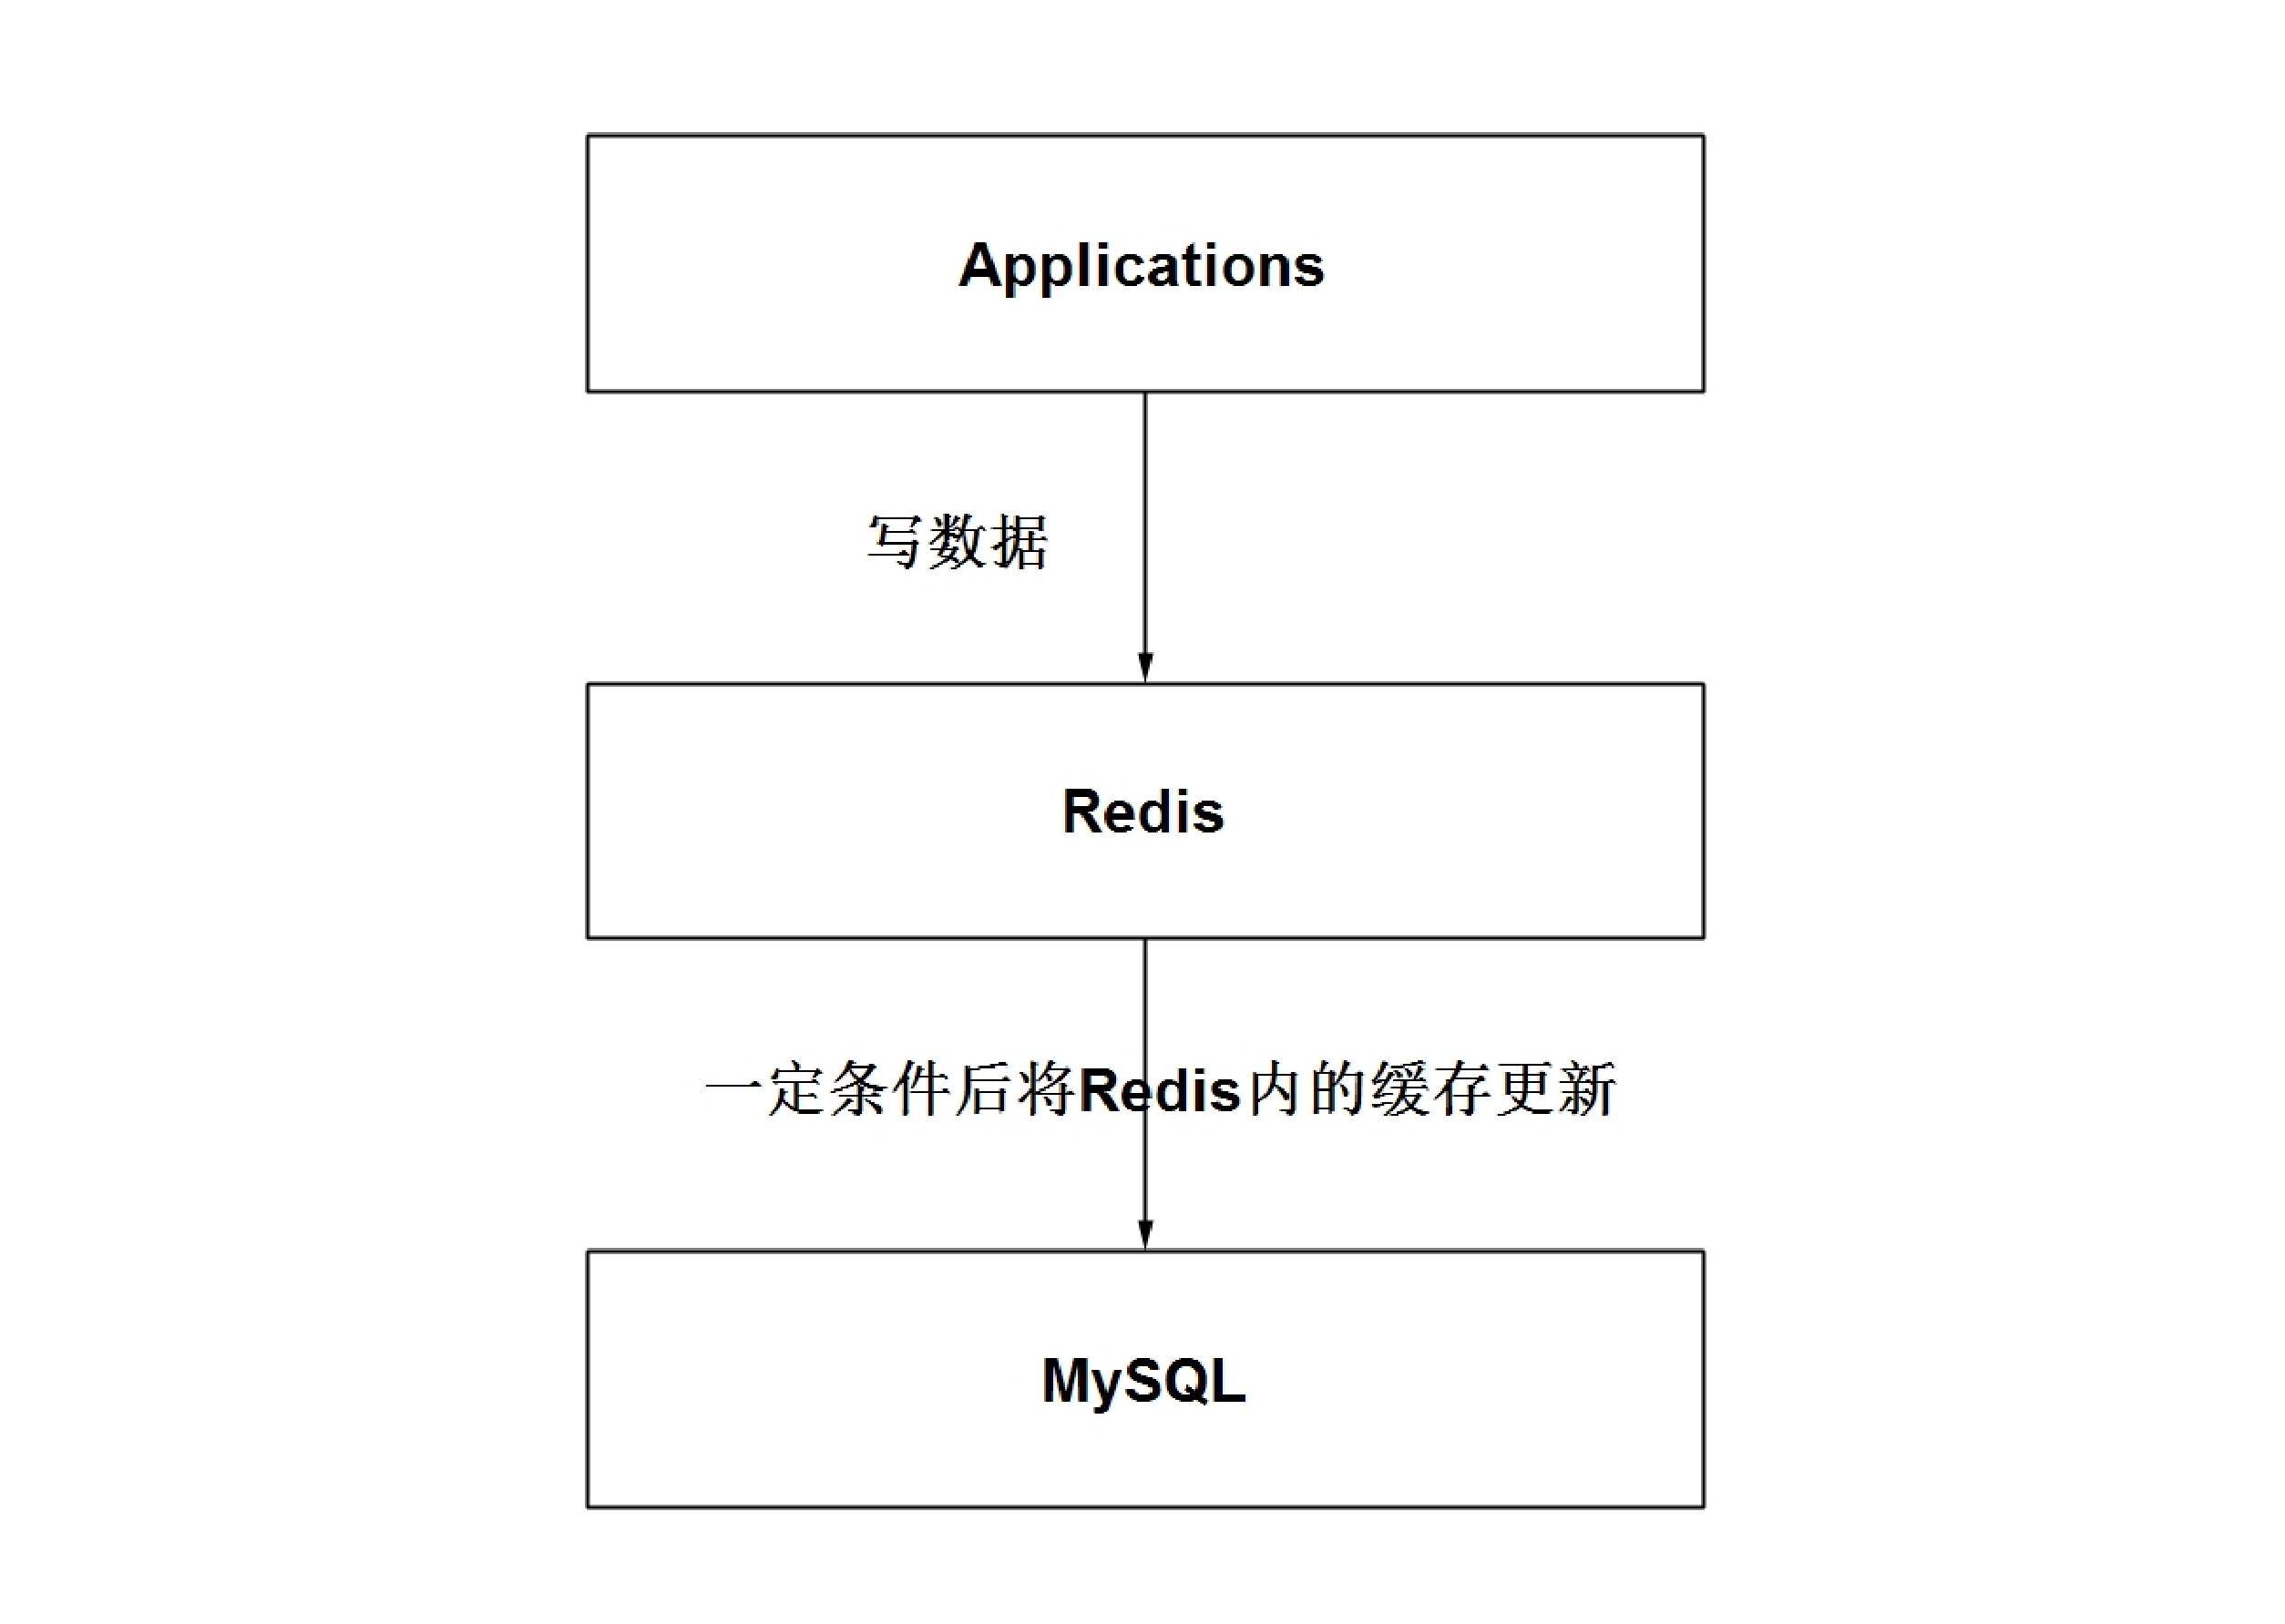
\includegraphics[width=0.4\textwidth]{redis1}
\caption{写架构}\label{fig:redis1}
\vspace{\baselineskip}
\end{figure}

\begin{figure}[htbp]
\centering
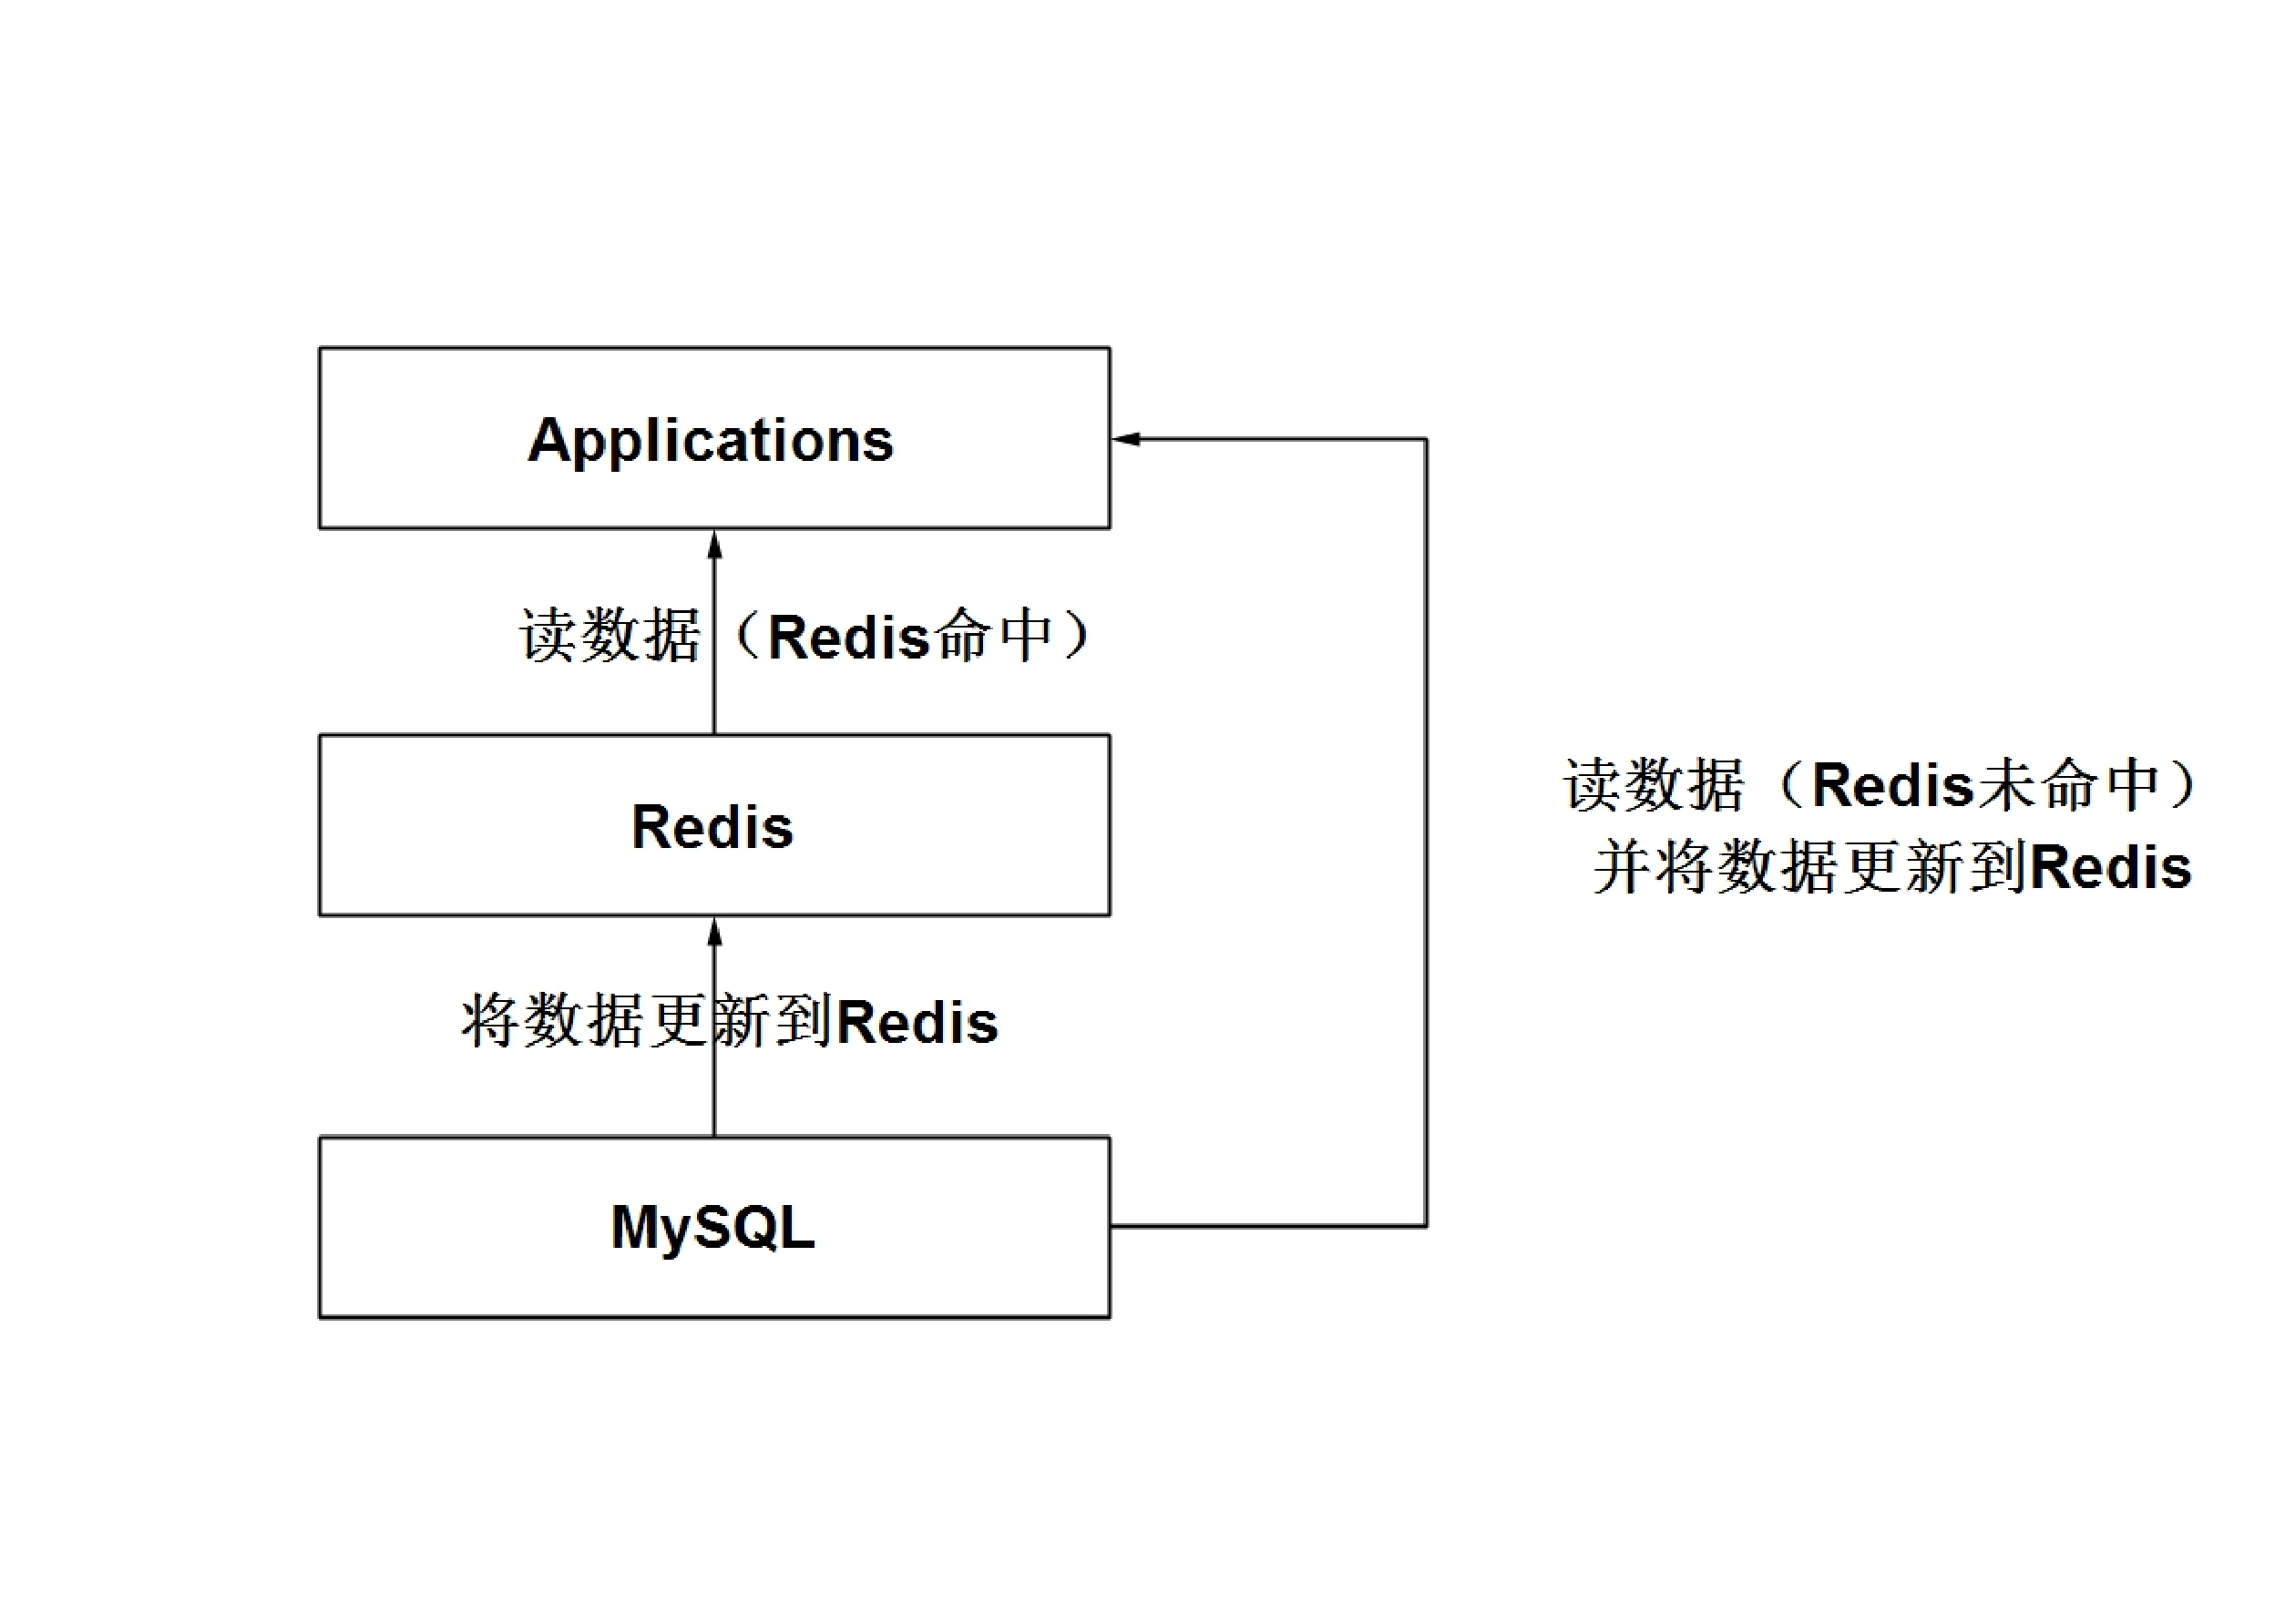
\includegraphics[width=0.4\textwidth]{redis2}
\caption{读架构}\label{fig:redis2}
\vspace{\baselineskip}
\end{figure}

}
\item{编程语言:Python\\

Python是一种面向对象、直译式计算机程序设计语言,由Guido van Rossum于1989年底发明,第一个公开发行版发行于1991年。Python语法简捷而清晰,具有丰富和强大的类库。它常被昵称为胶水语言,它能够很轻松的把用其他语言制作的各种模块(尤其是C/C++)轻松地联结在一起。

\begin{enumerate}[label=\Alph*.]
\item{简单:Python是一种代表简单主义思想的语言。阅读一个良好的Python程序就感觉像是在读英语一样。它使你能够专注于解决问题而不是去搞明白语言本身。}
\item{易学:Python极其容易上手,因为Python有极其简单的文档。}
\item{免费、开源:Python是FLOSS(自由/开放源码软件)之一。使用者可以自由地发布这个软件的拷贝、阅读它的源代码、对它做改动、把它的一部分用于新的自由软件中。FLOSS是基于一个团体分享知识的概念。}
\item{高层语言:用Python语言编写程序的时候无需考虑诸如如何管理你的程序使用的内存一类的底层细节。}
\item{可移植性:由于它的开源本质,Python已经被移植在许多平台上(经过改动使它能够工作在不同平台上)。这些平台包括Linux、Windows、FreeBSD、Macintosh、Solaris、OS/2、Amiga、AROS、AS/400、BeOS、OS/390、z/OS、Palm OS、QNX、VMS、Psion、Acom RISC OS、VxWorks、PlayStation、Sharp Zaurus、Windows CE、PocketPC、Symbian以及Google基于linux开发的android平台。}
\item{解释性:一个用编译性语言比如C或C++写的程序可以从源文件(即C或C++语言)转换到一个你的计算机使用的语言(二进制代码,即0和1)。这个过程通过编译器和不同的标记、选项完成。
运行程序的时候,连接/转载器软件把你的程序从硬盘复制到内存中并且运行。而Python语言写的程序不需要编译成二进制代码。你可以直接从源代码运行 程序。在计算机内部,Python解释器把源代码转换成称为字节码的中间形式,然后再把它翻译成计算机使用的机器语言并运行。这使得使用Python更加简单。也使得Python程序更加易于移植。}
\item{面向对象:Python既支持面向过程的编程也支持面向对象的编程。在“面向过程”的语言中,程序是由过程或仅仅是可重用代码的函数构建起来的。在“面向对象”的语言中,程序是由数据和功能组合而成的对象构建起来的。}
\item{可扩展性:如果需要一段关键代码运行得更快或者希望某些算法不公开,可以部分程序用C或C++编写,然后在Python程序中使用它们。}
\item{可嵌入性:可以把Python嵌入C/C++程序,从而向程序用户提供脚本功能。}
\item{丰富的库:Python标准库确实很庞大。它可以帮助处理各种工作,包括正则表达式、文档生成、单元测试、线程、数据库、网页浏览器、CGI、FTP、电子邮件、XML、XML-RPC、HTML、WAV文件、密码系统、GUI(图形用户界面)、Tk和其他与系统有关的操作。这被称作Python的“功能齐全”理念。除了标准库以外,还有许多其他高质量的库,如wxPython、Twisted和Python图像库等等。}
\item{规范的代码:Python采用强制缩进的方式使得代码具有较好可读性。而Python语言写的程序不需要编译成二进制代码。}
\end{enumerate}}

\item{数据库软件:MySQL}
\end{enumerate}

\chapter{研究工作总体安排与时间进度}
\begin{table}[htbp]
\caption{工作总体安排与时间进度}\label{tab:table1}
\vspace{0.5em}
\begin{center}
{\wuhao
\begin{tabular}{|c|c|c|}
\hline
任务序号 & 起止时间 & 阶段任务要点\\ \hline
1 & 2013.1.11~-~2013.2.20 & 了解课题相关内容,查找中、英文资料\\ \hline
2 & 2013.2.21~-~2013.3.8 & 查阅文献资料,完成文献综述、开题报告和外文翻译\\ \hline
3 & 2013.3.9~-~2013.3.25 & 阅读Redis源代码,分析其架构\\ \hline
4 & 2013.3.26~-~2013.4.1 & 系统详细设计\\ \hline
5 & 2013.4.2~-~2013.4.24 & 编码\\ \hline
6 & 2013.4.25~-~2013.4.30 & 系统测试\\ \hline
7 & 2013.5.1~-~2013.5.15 & 整理资料,完成论文\\ \hline
\end{tabular}}
\end{center}
\vspace{\baselineskip}
\end{table}

\backmatter
\endgroup % 组结束
%%%%%%%%%% 参考文献 %%%%%%%%%%
\clearpage % 显式换页,使书签定位准确
\bibliography{references/literaturereview_reference}
\nocite{*}                                   % 若将此命令屏蔽掉,则未引用的文献不会出现在文后的参考文献中。

%%%%%%%%%% 附录 %%%%%%%%%%
%\appendix
%\include{appendix/appendix}            % 附录

\end{document}                                  % 结束全文
